% +--------------------------------------------------------------------+
% | LaTeX Template                                                     |
% | for K-State Electronic Theses, Dissertations, and Reports          |
% |                                                                    |
% | Comments and guidelines for using the template are shown           |
% | within boxes like this one.                                        |
% |                                                                    |
% | Revised 6/30/06                                                    |
% | 9/14/06: Removed typos                                             |
% +--------------------------------------------------------------------+

% +--------------------------------------------------------------------+
% | Your paper should contain the following sections, except where     |
% | indicated as optional, in the order shown.  Also, all headings     |
% | shown with an asterisk (*) must be centered and in uppercase       |
% | letters:                                                           |
% |                                                                    |
% | Abstract Title Page (doctoral dissertations only)                  |
% | ABSTRACT* (doctoral dissertations only)                            |
% | Title Page                                                         |
% | Copyright Page (Optional - only needed if copyrighting)            |
% | ABSTRACT *                                                         |
% | TABLE OF CONTENTS *                                                |
% | LIST OF FIGURES *                                                  |
% | LIST OF TABLES*                                                    |
% | ACKNOWLEDGMENTS* (Optional)                                        |
% | DEDICATION * (Optional)                                            |
% | PREFACE * (Optional)                                               |
% | Individual Chapters                                                |
% | References and/or bibliography                                     |
% | Appendices (as needed)                                             |
% +--------------------------------------------------------------------+

% +--------------------------------------------------------------------+
% | The LaTex keyword \documentclass selects a particular class to     |
% | associate with the document.  The current documentclass            |
% | {class_diss} generates a Table of Contents that has leading dots   |
% | only on chapter subheadings.  If you prefer a Table of Contents    |
% | that has leading dots for all entries, replace {class_diss}        |
% | with {Mydiss} in the command below.                                |
% |                                                                    |
% +--------------------------------------------------------------------+

\documentclass[final, 12pt,oneside]{class_diss}

% +--------------------------------------------------------------------+
% | The following command sets the bibliography style to American
% | Institute of Physics (AIP).  Other styles are available in the
% | styles directory.  To use a different style, replace "aip" with
% | the filename of the style you want to use.
% +--------------------------------------------------------------------+

%\bibliographystyle{styles/plain}

\usepackage[utf8]{inputenc}
\usepackage[T1]{fontenc}
\usepackage[spanish]{babel}
\selectlanguage{spanish}
\usepackage{eurosym}

% +--------------------------------------------------------------------+
% | Now, we add in all external packages that we will use throughout   |
% | the document.  You can add other packages as needed.
% +--------------------------------------------------------------------+

%\usepackage{     caption2} % Customize captions a bit more
\usepackage{      amsmath} % American Mathematics Society standards
%\usepackage{      wrapfig} % Wraps text around a figure or table
\usepackage{     graphicx} % Extended graphics package.
%\usepackage{     fancyhdr} % Efficiently handles headers and footers
%\usepackage{       braket} % Bra-Ket notation package
%\usepackage{     mathrsfs} % Specialized Math fonts (Hamiltonian, etc.)
%\usepackage{boxedminipage} % Boxed text can be produced
%\usepackage{     setspace} % Controls line spacing via \begin{space}

\usepackage{amsxtra}
\usepackage{amssymb}
\usepackage{amsmath}
\usepackage{latexsym}
\usepackage{subfigure}
\usepackage{enumerate}
\usepackage{float}

% +--------------------------------------------------------------------+
% | The color package allows one to select colors for hyperlinking     |
% | (see below).                                                       |
% +--------------------------------------------------------------------+

\usepackage[usenames]{color}

% +--------------------------------------------------------------------+
% | Colors defined for use with this template.                         |
% +--------------------------------------------------------------------+

\definecolor{  Pink}{rgb}{1.0, 0.5, 0.5}
\definecolor{Maroon}{rgb}{0.8, 0.0, 0.0}

% +--------------------------------------------------------------------+
% | In the commands below, we use the 'natbib' package, and specify    |
% | the 'sort&compress' option, which condenses                        |
% | citations from (1,2,3,5,9,10,11) to (1-3,5,9-11).  The 'bibpunct'  |
% | option selects various parameters for how the citation will be     |
% | displayed.  In this case, only the comma (separation between       |
% | citations) and the 's' (superscript) arguments are chosen.  The    |
% | other curly braces deal with how to 'wrap' the citation (using     |
% | parentheses, brackets, etc.) and are not needed for the chosen     |
% | style.                                                             |
% +--------------------------------------------------------------------+

\usepackage[sort&compress]{natbib}
%\bibpunct{}{}{,}{s}{}{}
%\usepackage{hypernat}

% +--------------------------------------------------------------------+
% | Lastly, the hyperref package allows one to hyperlink cross-        |
% | references and figures in a LaTeX document.                        |
% +--------------------------------------------------------------------+

\usepackage[pdftex, plainpages=false, pdfpagelabels]{hyperref}
\usepackage{url}
\usepackage{listings}
%\usepackage{minted}
\hypersetup{
    linktocpage=true,
    colorlinks=true,
    bookmarks=true,
    citecolor=blue,
    urlcolor=red,
    linkcolor=Maroon,
    citebordercolor={1 0 0},
    urlbordercolor={1 0 0},
    linkbordercolor={.7 .8 .8},
    breaklinks=true,
    pdfpagelabels=true,
    }

% +--------------------------------------------------------------------+
% | Page margins are set on 1 inch on all sides.                       |
% +--------------------------------------------------------------------+

\topmargin      = -0.56in
\textheight     =  8.60in
\textwidth      =  6.46in
\oddsidemargin  =  0.02in

% +--------------------------------------------------------------------+
% | The document finally begins here.                                  |
% +--------------------------------------------------------------------+

\begin{document}


  \setcounter{page}{-1}


% +--------------------------------------------------------------------+
% | Title Page -- Required for both Doctoral and Masters Students
% +--------------------------------------------------------------------+

% +--------------------------------------------------------------------+
% | Title Page
% +--------------------------------------------------------------------+

\newpage

% +--------------------------------------------------------------------+
% | This page should not contain a page number.  We use the
% | \thispagestyle[empty] command below to suppress page numbers
% | and other style elements.
% +--------------------------------------------------------------------+

\thispagestyle{empty}

% +--------------------------------------------------------------------+
% | The Title page begins here.
% +--------------------------------------------------------------------+

\begin{center}

   \vspace{1cm}

% +--------------------------------------------------------------------+
% | On the line below, replace "ENTER YOUR TITLE" with the title of
% | your ETDR.  Use all CAPITAL LETTERS.
% +--------------------------------------------------------------------+

   {\Large \textbf{UNIVERSIDAD COMPLUTENSE DE MADRID}}\\

   \vspace{0.3cm}
   {\Large FACULTAD DE CIENCIAS FÍSICAS}\\
   \vspace{0.3cm}
   {DEPARTAMENTO DE Arquitectura de computadores y Automática}\\

   

   \vspace{0.65cm}
   \rule{2in}{0.5pt}\\
   \vspace{0.85cm}

\vspace{0.5cm}

  
\includegraphics[height=2.4in]{figures/escudo.jpg}

   \vspace{0.5cm}  
  {\large \textbf{TRABAJO DE FIN DE GRADO}}\\ 

  \vspace{0.3cm} 

  \textbf{Código TFG: [Código TFG]}\\
  
   \vspace{0.5cm}
     
%+-- Escribe el nombre de tu Trabajo de Fin de Grado
  \textbf{[Localización relativa de sensores con chips de banda ultra ancha]}\\
  \vspace{0.3cm}  
  \textbf{[Relative localization of sensors using ultra wideband chips]}
% +--------------------------------------------------------------------+

   \vspace{1.2cm}

% Nombre del alumno y datos de la convocatoria:   
  [Nombre del Alumno]\\

   \vspace{1.2cm}
% Supervisores o directores del trabajo:
  Supervisor/es: [Nombre del/os supervisores]
% +--------------------------------------------------------------------+   
  
  \vspace{2.5cm}
  Grado en Ingeniería Electrónica de Comunicaciones\\
  Curso académico 20[XX-XX]\\
  Convocatoria XXXX\\



\end{center}

%{\raggedleft
%Directores:\\
%   \vspace{ 1cm}
%Apellidos, Nombre\\
%Apellidos, Nombre\\
%}


% +--------------------------------------------------------------------+
% | Use the section below if you have co-major professors.
% +--------------------------------------------------------------------+

%\begin{flushleft}
%   \hspace{10cm}Approved by:\\
%   \vspace{ 1cm}
%   \hspace{10cm}Co-Major Professor\\
%   \hspace{10cm}Enter Your Co-Major Professor's Name\\
%   \vspace{.5cm}
%   \hspace{10cm}Co-Major Professor\\
%   \hspace{10cm}Enter Your Co-Major Professor's Name\\
%\end{flushleft}

   \pdfbookmark[0]{Portada}{PDFPortadaPage}

% +--------------------------------------------------------------------+
% | Autorizacion Page -- Required for both Doctoral and Masters Students
% +--------------------------------------------------------------------+

% +--------------------------------------------------------------------+
% | Copyright Page
% +--------------------------------------------------------------------+
% 
\newpage
\thispagestyle{empty}
\mbox{}
\newpage

\thispagestyle{empty}

\begin{center}

{\bf \Huge Autorización de difusión}

\vspace{1cm}

% +--------------------------------------------------------------------+
% | On the line below, replace "Enter Your Name" with your name Use the same
% | form of your name as it appears on your title page. Use mixed case, for
% | example, Lori Goetsch.
% +--------------------------------------------------------------------+
% 
   \large Apellidos, Nombre\\

   \vspace{0.5cm}

% +--------------------------------------------------------------------+
% | On the line below, replace Fecha
% | % |
% +--------------------------------------------------------------------+
% 
   Madrid, a XX de XX de XX\\

   \vspace{0.5cm} \end{center}

Los abajo firmantes, matriculados en el Grado de XX de la
Facultad de XX, autorizan a la Universidad Complutense de Madrid (UCM) a
difundir y utilizar con fines académicos, no comerciales y mencionando
expresamente a su autor el presente Trabajo Fin de Grado: “Título”, realizado
durante el curso académico XX-XX bajo la dirección de XX y la co-dirección de XX en el Departamento de XX, y a la
Biblioteca de la UCM a depositarlo en el Archivo Institucional E-Prints
Complutense con el objeto de incrementar la difusión, uso e impacto del trabajo
en Internet y garantizar su preservación y acceso a largo plazo.

{
\begin{center}
\vfill

\includegraphics{figures/cc-by-nc-sa.png}
\tiny

Esta obra está bajo una\\
\href{http://creativecommons.org/licenses/by-nc-sa/4.0/}{Licencia Creative Commons\\Atribución-NoComercial-CompartirIgual 4.0 Internacional}.
\end{center}
}
   \pdfbookmark[0]{Autorización}{PDFAutorizacionPage}


% +--------------------------------------------------------------------+
% | Dedication Page
% |
% | If you choose not to have a Dedication page, comment out
% | or delete the following 3 lines.
% +--------------------------------------------------------------------+

\newpage
\vspace{1cm}
\setlength{\baselineskip}{0.8cm}

\begin{flushright}
\textit{``Dedicatoria, si es necesaria.''
}\\
Edward Tufte
\end{flushright}
\phantomsection
%\addcontentsline{toc}{chapter}{Dedicatoria}

   % +--------------------------------------------------------------------+
% | Acknowledgements Page
% |
% | If you choose not to have an Acknowledgements page, comment out
% | or delete the following 3 lines.
% +--------------------------------------------------------------------+

\newpage
\begin{center}
{\bf \Huge Agradecimientos}
\end{center}
\vspace{1cm}
\setlength{\baselineskip}{0.8cm}

\begin{flushright}
\textit{Agradecimientos, si son necesarios.
}
\end{flushright}


\phantomsection
%\addcontentsline{toc}{chapter}{Agradecimientos}

% +--------------------------------------------------------------------+
% | We use the following code to suppress page numbers and other
% | style issues we do not want present on a given page.               |
% +--------------------------------------------------------------------+

%\thispagestyle{empty} Looks like it's ok to remove this line
\newpage
\pagenumbering{roman}

% +--------------------------------------------------------------------+
% | On the line below, set the number to represent the page number of
% | the Table of Contents page.  For example, if the Table of Contents
% | page is the 8th page of your document, enter 8 in the brackets.  This
% | number may vary, depending on the length of your abstract.
% |
% | Numbers do not appear on the title and abstract pages, but they are
% | included in the page count.  The Table of Contents page is the
% | first page on which page numbers are displayed.
% +--------------------------------------------------------------------+

\setcounter{page}{1}


% +--------------------------------------------------------------------+
% | Preface Page (Prologo)
% +--------------------------------------------------------------------+

%% EN PRINCIPIO NO LO USAMOS

% +--------------------------------------------------------------------+
% | Preface (Optional)
% +--------------------------------------------------------------------+

\newpage
\begin{center}
{\bf \Huge Preface}
\end{center}
\vspace{1cm}
\setlength{\baselineskip}{0.8cm}

%\pdfbookmark[0]{Preface}{PDF_Preface}

% +--------------------------------------------------------------------+
% | Enter text of your Preface in the space below this box.
% +--------------------------------------------------------------------+

This template uses a separate file for each section of your ETDR:
title page, abstract, preface, chapters, reference, etc.  This
makes it easier to organize and work with a lengthy document.  The
template is configured with page margins required by the Graduate
School and will automatically create a table of contents, lists of
tables and figures, and PDF bookmarks.

Although the template gives you a foundation for creating your
ETDR, you will need a working knowledge of LaTeX in order to
produce a final document.  You should be familiar with LaTeX
commands for formatting text, equations, tables, and other
elements you will need to include in your ETDR.

This template uses a separate file for each section of your ETDR:
title page, abstract, preface, chapters, reference, etc.  This
makes it easier to organize and work with a lengthy document.  The
template is configured with page margins required by the Graduate
School and will automatically create a table of contents, lists of
tables and figures, and PDF bookmarks.

Although the template gives you a foundation for creating your
ETDR, you will need a working knowledge of LaTeX in order to
produce a final document.  You should be familiar with LaTeX
commands for formatting text, equations, tables, and other
elements you will need to include in your ETDR.

This template uses a separate file for each section of your ETDR:
title page, abstract, preface, chapters, reference, etc.  This
makes it easier to organize and work with a lengthy document.  The
template is configured with page margins required by the Graduate
School and will automatically create a table of contents, lists of
tables and figures, and PDF bookmarks.

Although the template gives you a foundation for creating your
ETDR, you will need a working knowledge of LaTeX in order to
produce a final document.  You should be familiar with LaTeX
commands for formatting text, equations, tables, and other
elements you will need to include in your ETDR.

%\phantomsection
%\addcontentsline{toc}{chapter}{Preface}

% +--------------------------------------------------------------------+
% | Here, we will generate our Table of Contents (TOC) entries.        |
% | This adds the section to the TOC and then generates the indicated  |
% | section.                                                           |
% +--------------------------------------------------------------------+



\phantomsection
\addcontentsline{toc}{chapter}{Índice}

\tableofcontents
\listoffigures
%\listoftables

%\hfill  Are these lines necessary?
%\hfill

\newpage
\addcontentsline{toc}{chapter}{Resumen}
\pdfbookmark[0]{Resumen}{PDFResumenPage}
% +--------------------------------------------------------------------+
% | Copyright Page
% +--------------------------------------------------------------------+

\newpage

\thispagestyle{empty}

{\bf \large [Título extendido del TFG (si procede)]}

\vspace{0.5cm}

{\bf \large Resumen}\\
Breve resumen de contenidos.


\vspace{5cm}


{\bf Palabras clave:}


   
   Separadas, por, comas.
   
   \vspace{1 cm}


{\bf \large Abstract}\\

\vspace{5cm}

{\bf Key works:}

% ------------- Para eliminar ----------
\vspace{0.9cm}
\begin{center}
[Nota: el título extendido (si procede), el resumen y abstract deben estar en una misma página y su extensión no debe superar la página. Tamaño mínimo 11 pto.\\

Extensión máxima 50 páginas sin contar portada ni resumen (sí se incluye índice, introducción, conclusiones y bibliografía)]\\
\end{center}
% ----------------------------------------
  

%   % +--------------------------------------------------------------------+
% | Copyright Page
% +--------------------------------------------------------------------+

\newpage

\thispagestyle{empty}

\begin{center}

{\bf \Huge Resumen}

  \end{center}
\vspace{1cm}

Breve resumen de contenidos.


\vspace{1cm}

% +--------------------------------------------------------------------+
% | On the line below, repla	ce Fecha
% |
% +--------------------------------------------------------------------+

\begin{center}

{\bf \Large Palabras clave}

   \end{center}

   \vspace{0.5cm}
   
   Separadas, por, comas.
   




%   \addcontentsline{toc}{chapter}{Resumen}
%   \pdfbookmark[0]{Resumen}{PDFResumenPage}

%    % +--------------------------------------------------------------------+
% | Copyright Page
% +--------------------------------------------------------------------+

\newpage

\thispagestyle{empty}

\begin{center}

{\bf \Huge Abstract}

  \end{center}
\vspace{1cm}


 
\vspace{1cm}

% +--------------------------------------------------------------------+
% | On the line below, replace Fecha
% |
% +--------------------------------------------------------------------+

\begin{center}

{\bf \Large Keywords}

   \end{center}

   \vspace{0.5cm}
   
Separadas, por, comas.
   



%       \addcontentsline{toc}{chapter}{Abstract}
%       \pdfbookmark[0]{Abstract}{PDFAbstractPage}
%   \vfill
    
    



% +--------------------------------------------------------------------+
% | We use arabic (1, 2, 3...) page numbering starting from page 1.    |
% | Note, however, that there are many pages where this is not the     |
% | desired behavior - such as the Title page, or abstract.  In these  |
% | cases, we can use \thispagestyle{empty} to suppress page numbers,  |
% | and other general style issues that we've defined globally.        |
% +--------------------------------------------------------------------+

\newpage
\pagenumbering{arabic}
\setcounter{page}{1}

% +--------------------------------------------------------------------+
% | Here is where we include individual sections of the thesis or
% | dissertation.                                                      |
% +--------------------------------------------------------------------+

% +--------------------------------------------------------------------+
% | Chapters
% +--------------------------------------------------------------------+

% -----------Incluir esto en caso necesario para que el capítulo comience siempre en página impar

%\newpage
%\thispagestyle{empty}
%\mbox{}
%---------------------------------------

\chapter{Introducción}
\label{ch:chapter1}

\section{Motivación}


\section{Estado del arte}

\section{Organización de la memoria}

Tengo que preguntar en que parte ira el sustento teorico de las cosas en las que hable en el capitulo 2


% +--------------------------------------------------------------------+
% | Uncomment the lines below to add additional chapters.  Name the
% | files chapter2.tex for Chapter 2, chapter3.tex for Chapter 3, etc.
% +--------------------------------------------------------------------+


\newpage
\thispagestyle{empty}
\mbox{}
\setlength{\parskip}{4mm}
\chapter{Algoritmos de Localización}
\label{ch:chapter2}


Todos los sistemas a continuación serán descritos desde el punto de vista de sistemas en variables de estado. Para los modelos utilizados los vehículos se interpretan como masas puntuales en el espacio centrados en el centro de masa de estos. Con esto en consideración se puede pasar.

\section{Descripción de un vehículo como modelo continuo}
\par
Considerando que los vehículos autónomos tienen como entrada su velocidad y se puede cuantificar su magnitud en el eje X e Y con lo que la evolución de la posición del vehículo en este eje de coordenadas es descrita con el siguiente sistema. 
\begin{equation*}
\left.
 \begin{aligned}
P_{x_1}(t) & = P_{x_1}(0)+V_{x_1}(t)\cdot t \\
P_{y_1}(t) & = P_{y_1}(0)+V_{y_1}(t)\cdot t
\end{aligned}
\right\}
\quad\text{Sistema de un vehiculo continuo}
\end{equation*}
\par
Esto es considerando que se esta tratando con un sistema continuo, sin embargo, al tratarse de sistemas digitales este modelo deja de ser válido y se tendrá que pasar al siguiente. 
\begin{equation*}
\left.
 \begin{aligned}
P_{x_1}(k+1) & = P_{x_1}(k)+V_{x_1}(k)\cdot\Delta{T} \\
P_{y_1}(k+1) & = P_{y_1}(k)+V_{y_1}(k)\cdot\Delta{T} 
\end{aligned}
\right\}
\quad\text{Sistema de un vehículo discreto}
\end{equation*}
\par
En este sistema se tendrá como estado $q(k)=[P_{x1},P_{y1}]$ lo que implicará que la matriz F simplemente será la matriz identidad. Las entradas del sistema a su vez serán $u(k)=[V_{x1},V_{y1}]$.
No se discutirá todavía sobre la matriz H, esto se tratará en el apartado de corrección de la medida. 
Ahora se tendrá que tomar en consideración la incertidumbre de todos los componentes del sistema. Debido a que los instrumentos de medida tienen una determinada precisión no se podrá conocer con exactitud ni la posición, ni la velocidad del vehículo. Esto puede dar lugar a que el sistema antes descrito llegue a alejarse considerablemente de la realidad. 
\par
Para tomar esto en consideración se sustituirán los estados por elegidos por distribuciones gausianas cuya media corresponderá con la posición estimada del vehículo y la varianza nos dará información de con que probabilidad estará el vehículo dentro de una determinada región. De tal forma que la posición y velocidad real del vehículo seguirán la siguiente distribución. 
\begin{equation*}
\left.
 \begin{aligned}
P_{x_1}(x) & = \frac{1}{\sigma\sqrt{2\pi}} 
  \exp\left( -\frac{1}{2}\left(\frac{x-\hat{P_{x_1}}}{\sigma}\right)^{\!2}\,\right) \\
P_{y_1}(y) & = \frac{1}{\sigma\sqrt{2\pi}} 
  \exp\left( -\frac{1}{2}\left(\frac{y-\hat{P_{y_1}}}{\sigma}\right)^{\!2}\,\right)
\end{aligned}
\right\}
\quad\text{Distribución de la posición de un vehículo}
\end{equation*}

\begin{equation*}
\left.
 \begin{aligned}
V_{x_1}(x) & = \frac{1}{\sigma\sqrt{2\pi}} 
  \exp\left( -\frac{1}{2}\left(\frac{x-\hat{V_{x_1}}}{\sigma}\right)^{\!2}\,\right) \\
V_{y_1}(y) & = \frac{1}{\sigma\sqrt{2\pi}} 
  \exp\left( -\frac{1}{2}\left(\frac{y-\hat{V_{y_1}}}{\sigma}\right)^{\!2}\,\right)
\end{aligned}
\right\}
\quad\text{Distribución de la velocidad de un vehículo}
\end{equation*}

\par
Esto se puede hacer debido a que la suma de dos distribuciones gausianas independientes tiene la propiedad de que la media resultante será $\mu_{x+y}=\mu_{x}+\mu_{y}$ y la varianza $\sigma_{x+y}^2=\sigma_{x}^2+ \sigma_{y}^2$. Esto implica que el sistema seguirá siendo lineal. Se añadirá una matriz adicional que tomara en cuenta la evolución de la incertidumbre de (aumentara con el tiempo) y la media de estas gausianas sustituirán los estados. 
\par
En este punto se hace la distinción entre posición y velocidad real y posición estimada, siendo la posición estimada la que se determina con el sistema anteriormente descrito. Con esto los nuevos estados $\hat{q}(k)=[\hat{P_{x1}},\hat{P_{y1}}]$ y las entradas $\hat{u}(k)=[\hat{V_{x1}},\hat{V_{y1}}]$.
\par
En este punto se puede comparar la trayectoria estimada del vehículo con una de las trayectorias reales posibles que se pueden generar con el modelo utilizado. El primer caso para analizar es tener una posición inicial real diferente a la estimada, es decir que $q(0)\neq\hat{q}(0)$. Como se observa en la siguiente figura esta diferencia no tiene mucha influencia en la posición final del vehículo.  
\par

\begin{figure}[htb]
\centering
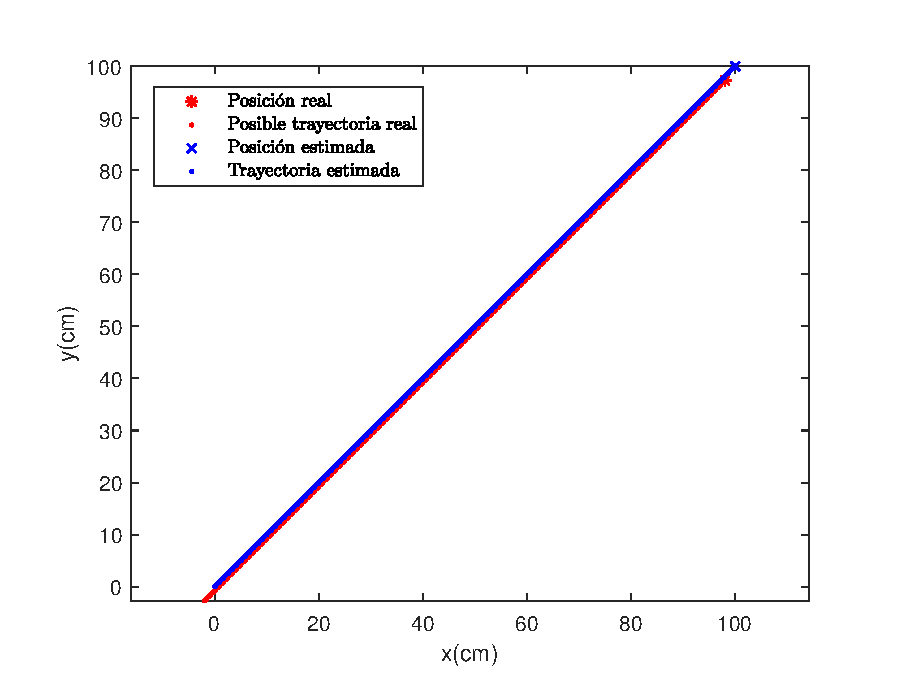
\includegraphics[width=0.8\textwidth]{figures/Figura-de-desviación-de-un-vehiculo-con-posición-incial-deferente-a-la-real.eps}
\caption{Diferencia entre trayectoria estimada y trayectoria real para posiciones iniciales diferentes} \label{fig:Pini_dif}
\end{figure}

Otro caso sencillo por analizar es que ocurre para una entrada constante (velocidad constante) donde $u(0)\neq\hat{u}(0)$.

\begin{figure}[htb]
\centering
\includegraphics[width=0.8\textwidth]{figures/Figura-de-desviación-de-un-vehiculo-con-velocidad-inicial-diferente-a-la-real.eps}
\caption{Diferencia entre trayectoria estimada y trayectoria real para velocidades iniciales diferentes} \label{fig:Vini_dif}
\end{figure}
\par 

En este caso el error es acumulativo y la diferencia entre la posición inicial y la posición final es significativa, por esta razón se debe recurrir a métodos de corrección para tener en consideración este tipo de incertidumbre. 

\section{Corrección utilizando el filtro de Kalman.}
Como se observo en una sección anterior la actualización de la incertidumbre del sistema se toma en cuenta en la matriz P a través de la siguiente expresión 
\begin{equation*}
\left.
 \begin{aligned}
P(k+1)&=FP(k)F'+GQG'
\end{aligned}
\right.
\end{equation*}
Donde la matriz Q es la matriz de covarianza de la entrada.
\par
En este punto es donde se hará uso de la relación de la salida del sistema de variables de estado con los propios estados del sistema 
\begin{equation*}
\left.
 \begin{aligned}
y(k)&=H\cdot{q(k)}
\end{aligned}
\right.
\end{equation*}
Se llamará H a la matriz de medida. En el caso más sencillo la medida obtenida será $P_{x1}$ y $P_{y1}$ quedando la matriz H como:
\begin{equation*}
\left.
 \begin{aligned}
H=\begin{pmatrix}
1 & 0\\
0 & 1 
\end{pmatrix}
\end{aligned}
\right.
\end{equation*}
Quedando así la salida del sistema estimada como:
\begin{equation*}
\left.
 \begin{aligned}
\hat{y}(k)=\begin{pmatrix}
1 & 0\\
0 & 1 
\end{pmatrix}\begin{pmatrix}
\hat{P_{x1}}\\
\hat{P_{y1}} 
\end{pmatrix}
\end{aligned}
\right.
\end{equation*}
Para realizar la corrección en de los estados se realiza la siguiente operación 
\begin{equation*}
\left.
 \begin{aligned}
\hat{q}(k)&=\hat{q}(k)+K\cdot{(y_{m}-\hat{y}(k))}
\end{aligned}
\right.
\end{equation*}
Siendo $y_{m}$ en este caso $\begin{pmatrix}
P_{x1}\\
P_{y1} 
\end{pmatrix}$, es decir la posición real del objeto, y K la ganancia del filtro de Kalman. 
También utilizando esta misma matriz H se actualiza la matriz de covariaza. 
\begin{equation*}
\left.
 \begin{aligned}
P=P-K·H·P
\end{aligned}
\right.
\end{equation*}
Cabe destacar que como las mediciones no están ligadas de ninguna manera la matriz P será diagonal todo el tiempo y los autovalores de esta matriz definirán los ejes de una elipse centrada en $[\hat{P_{x1}},\hat{P_{y1}}]$. Esta elipse indica el área en el que se puede encontrar el vehículo con un 68\% de probabilidad (una desviación típica). 
\par 

%\begin{figure}[h!]
%\centering
%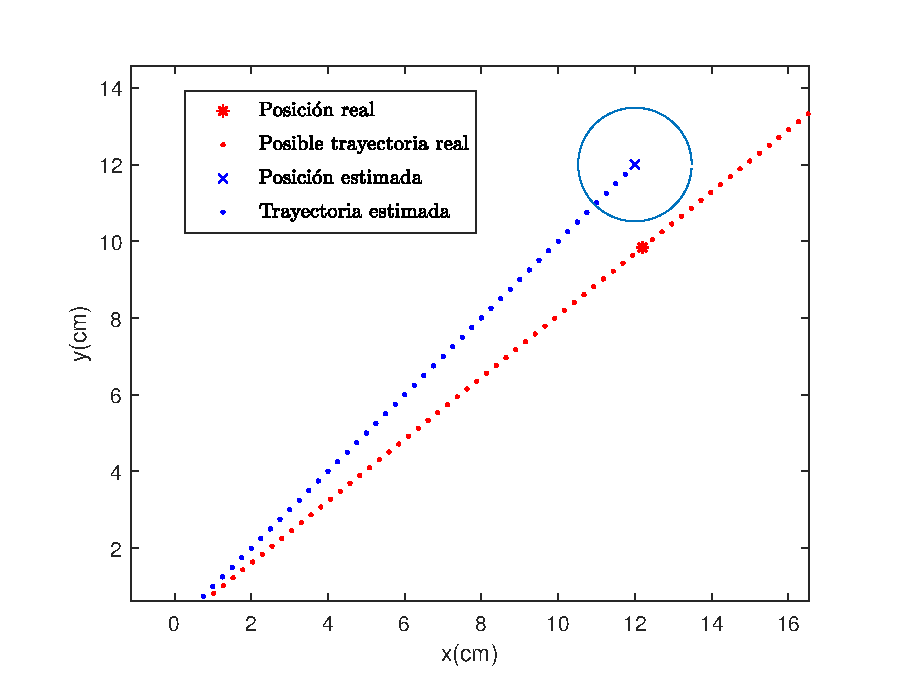
\includegraphics[width=0.8\textwidth]{figures/GraficarUnicarAntesdecorreccion.eps}
%\caption{Estado del sistema previo a una corrección} 
%\label{fig:Unicar_pre}
%\end{figure}
%\par 
%\begin{figure}[h!]
%\centering
%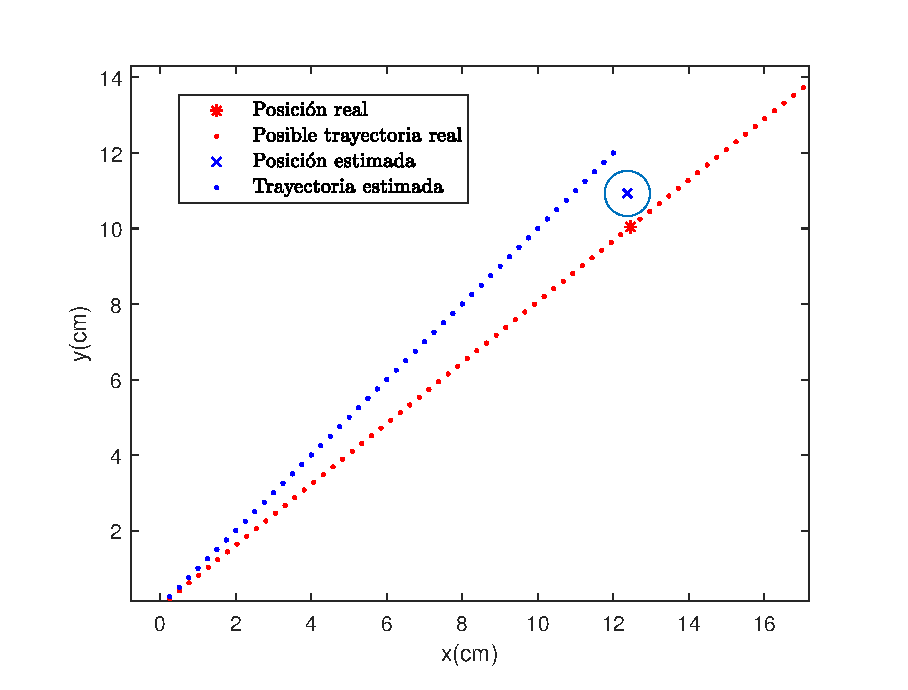
\includegraphics[width=0.8\textwidth]{figures/GraficarUnicardespuescorreccion.eps}
%\caption{Estado del sistema previo a una corrección} 
%\label{fig:Unicar_post}
%\end{figure}
%\par 



Sin embargo, por la restricción de hardware impuestas hacer una corrección individual de la posición global en X e Y no es posible. Únicamente se dispondrán de las distancias entre dos vehículos. Por lo que el sistema mínimo para obtener correcciones son dos vehículos. 
\newpage

\begin{figure}[!htb]
  \begin{center}
    \subfigure[Previo a corrección]{
        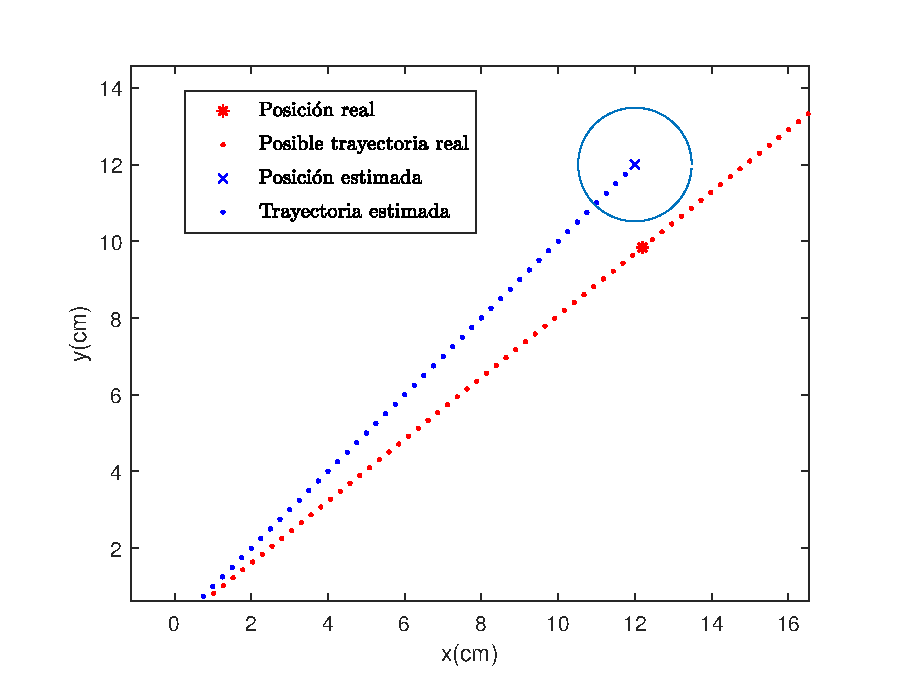
\includegraphics[width=0.7\textwidth]{figures/GraficarUnicarAntesdecorreccion.eps}
        \label{subfig:Unicar_pre}}
    \subfigure[Después de corrección]{
        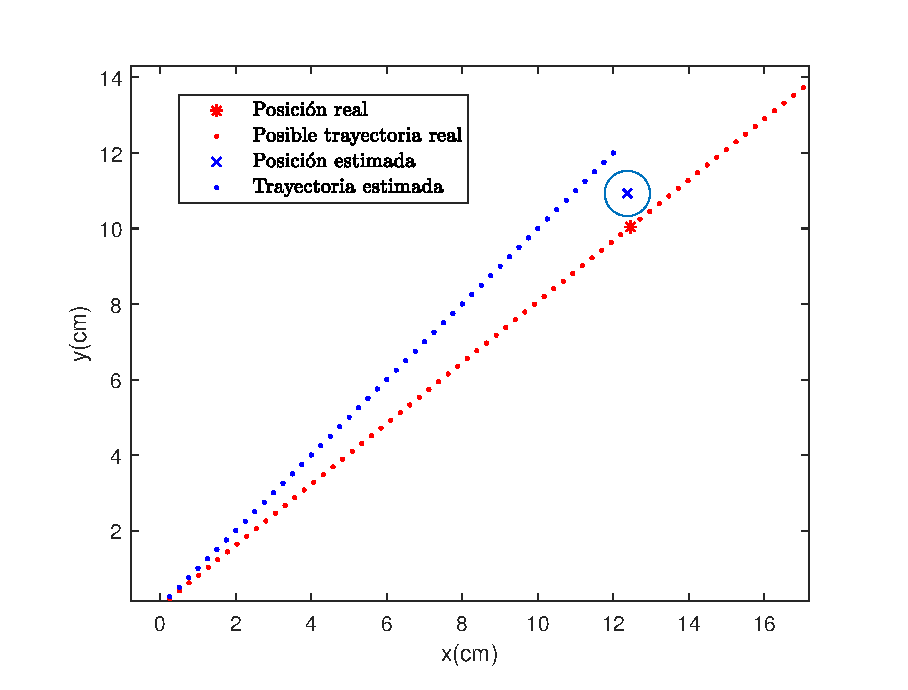
\includegraphics[width=0.7\textwidth]{figures/GraficarUnicardespuescorreccion.eps}
        \label{subfig:Unicar_pos}}
    \caption{Corrección con filtro de Kalman:Antes y después}
    \label{fig:CorrciónUnicar}
  \end{center}
\end{figure}
\newpage

\section{Extensión a dos vehículos}
El sistema de dos vehículos es una simple extensión del sistema de 1 vehículo

\begin{equation*}
\left.
 \begin{aligned}
P_{x_1}(k+1) & = P_{x_1}(k)+V_{x_1}(k)\cdot\Delta{T} (1) \\
P_{y_1}(k+1) & = P_{y_1}(k)+V_{y_1}(k)\cdot\Delta{T} (2)\\
P_{x_2}(k+1) & = P_{x_2}(k)+V_{x_2}(k)\cdot\Delta{T} (3)\\
P_{y_2}(k+1) & = P_{y_2}(k)+V_{y_2}(k)\cdot\Delta{T} (4)
\end{aligned}
\right\}
\quad\text{Sistema de dos vehiculos}
\end{equation*}
\par
Sin embargo al tener distancias la corrección se tiene que hacer en coordenadas relativas respecto a uno de los vehículos. Eligiendo que el punto de referencia es el vehículo 1 se consigue el sistema en coordenadas relativas simplemente restando la ecuación (1) a la (3) y la ecuación (2) a la (4) obteniendo:

\begin{equation*}
\left.
 \begin{aligned}
P_{x_21}(k+1) & = P_{x_21}(k)+V_{x_21}(k)\cdot\Delta{T} \\
P_{y_21}(k+1) & = P_{y_21}(k)+V_{y_21}(k)\cdot\Delta{T} 
\end{aligned}
\right\}
\quad\text{Sistema de un vehículo discreto}
\end{equation*}
\par
Se elige unas velocidades arbitrarias y se simulan ambos sistemas obteniéndose la figura \ref{fig:2CarAbs-Rel}. Cabe destacar que en este punto todavía no se consideran incertidumbres, solo se compara la evolución del sistema pasando de un eje de coordenadas a otro.
\par 
Ahora tomando en consideración que se trabaja con distribuciones y restas de distribuciones gausianas las incertidumbres del sistema pasaran a ser $\sigma_{21}^2=\sigma_{1}^2+\sigma_{2}^2$. Esto afectara la evolución de la matriz de covarianza P y por ende se traducirá en que se tendrá una mayor incertidumbre de donde estará un vehículo respecto al otro. 
\newpage
\begin{figure}[htb]
\centering
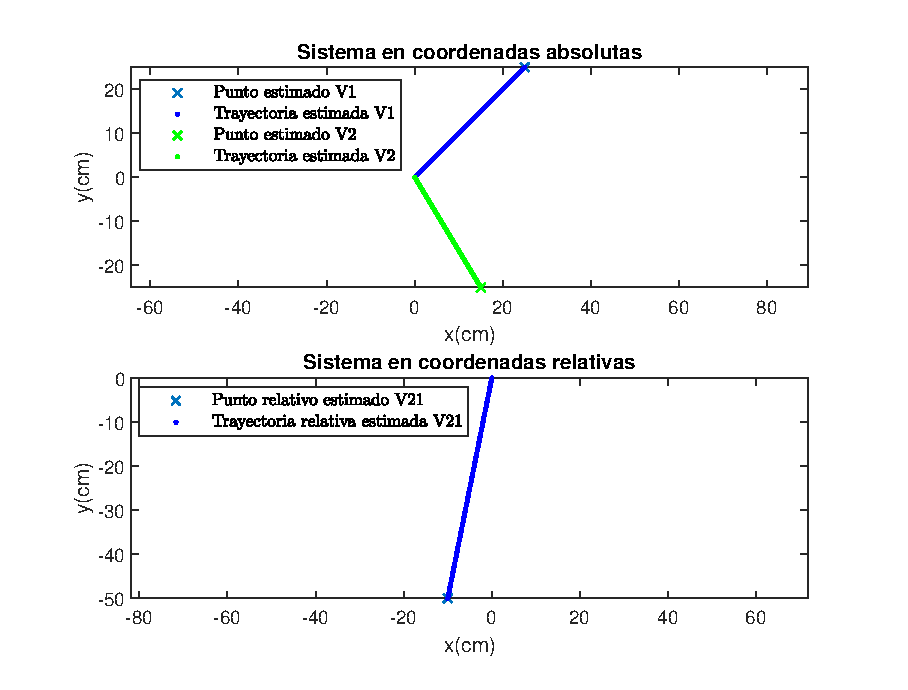
\includegraphics[width=0.8\textwidth]{figures/Sistema2CarAbs-Rel.eps}
\caption{Comparación de sistema en coordenas absolutas frente a relativas} 
\label{fig:2CarAbs-Rel}
\end{figure}
\par 

Ahora tomando en consideración que se trabaja con distribuciones y restas de distribuciones gausianas las incertidumbres del sistema pasaran a ser $\sigma_{21}^2=\sigma_{1}^2+\sigma_{2}^2$. Esto afectara la evolución de la matriz de covarianza P y por ende se traducirá en que se tendrá una mayor incertidumbre de donde estará un vehículo respecto al otro. 
\par
Una vez establecido el sistema en coordenadas relativas se puede realizar la corrección con la distancia. Hacer la corrección con la distancia tendrá dos implicaciones.
\begin{itemize}
	\item Al ser una combinación de la posición relativa en X y en Y (estados $\hat{P_{x_{21}}}$ y $\hat{P_{y_{21}}}$) al realizar la corrección estos estados estarán ligados por lo que la matriz P dejara de ser diagonal. 
	\item Es una combinación no lineal de los estados por lo que la matriz H se tendrá que ajustar a este hecho. 
\end{itemize}
Por último, hacer una corrección con una sola distancia presenta ambigüedad puesto a que si el segundo se encuentra en cualquier posición dentro del círculo de radio $d_{21}$, se detectara como que la trayectoria estimada es correcta a pesar de que el vehículo se puede estar desplazando en una dirección opuesta a la trayectoria real. 

\begin{figure}[htb]
\centering
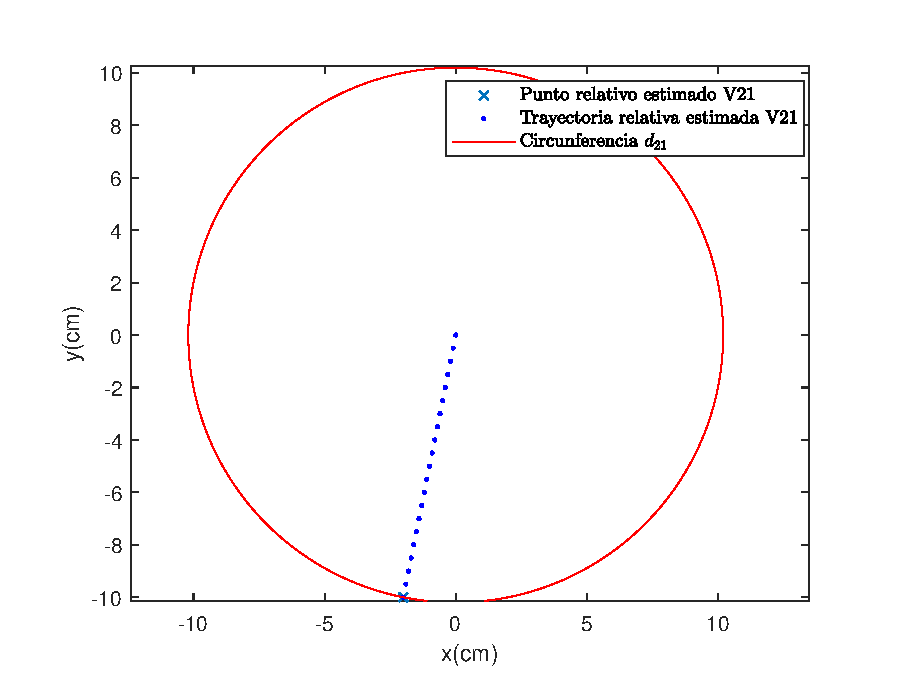
\includegraphics[width=0.8\textwidth]{figures/RadioAmbiguedad.eps}
\caption{Circunferencia correspondiente a $d_{21}$} 
\label{fig:Ambiguedad_1d}
\end{figure}
\par 

En la figura \ref{fig:Ambiguedad_1d} se muestra todos los puntos que tendrán una salida igual utilizando la matriz H discutida anteriormente. Ahora si se plantea un caso posible donde la velocidad real del vehículo difiere de la velocidad estimada de tal manera que la distancia sea la misma para ambas se podrá observar la consecuencia de solo tener una corrección con solo una medida de distancia \ref{fig:Correción2car}. 

\begin{figure}[!htb]
  \begin{center}
    \subfigure[Previo a corrección]{
        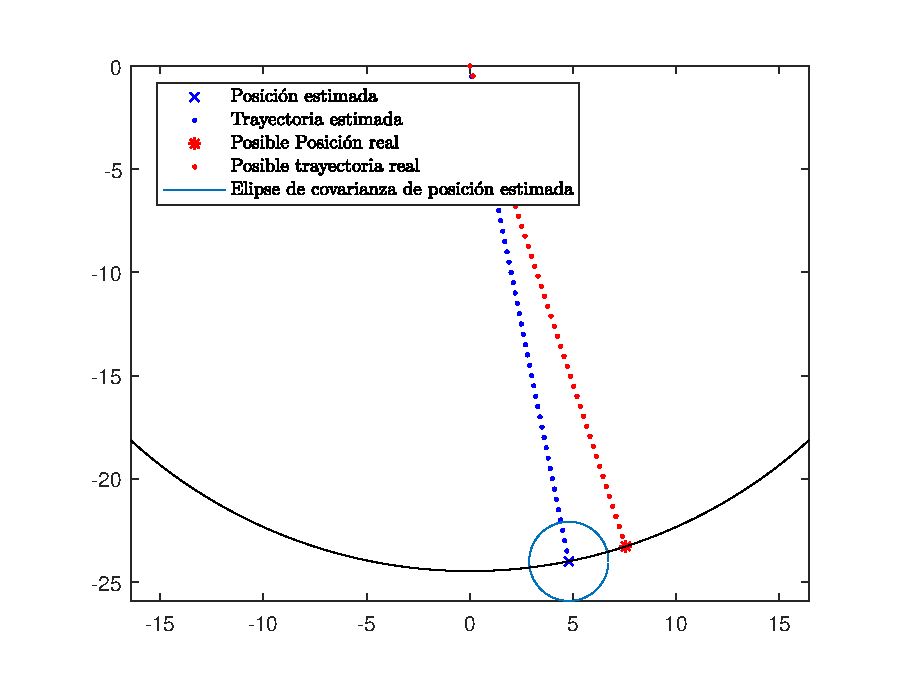
\includegraphics[width=0.7\textwidth]{figures/AmbiguedadPrecorreccion.eps}
        \label{subfig:2car_pre}}
    \subfigure[Después de corrección]{
        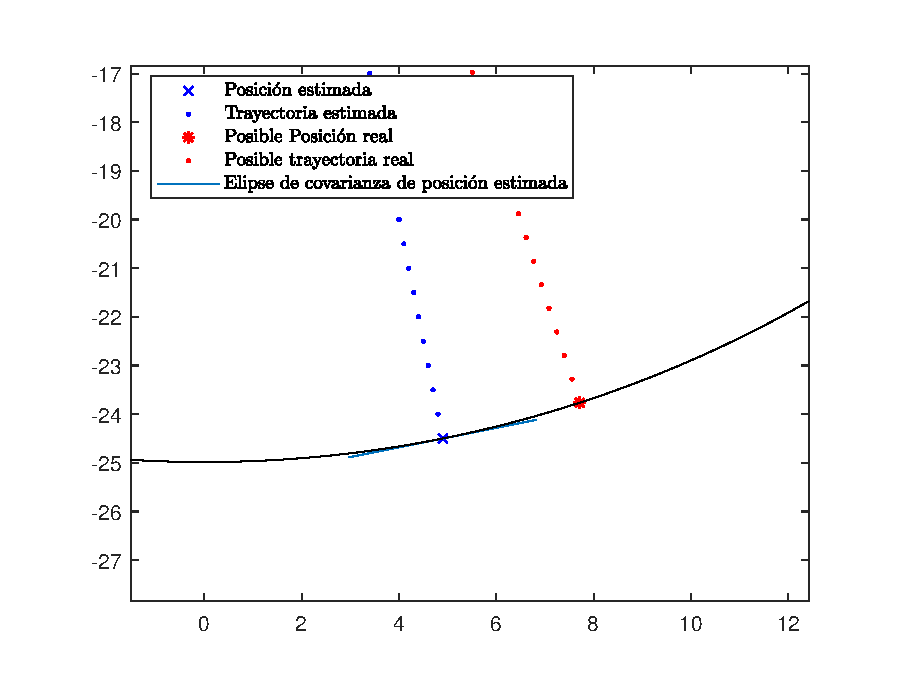
\includegraphics[width=0.7\textwidth]{figures/AmbiguedadPostcorreccion.eps}
        \label{subfig:2car_pos}}
    \caption{Corrección con filtro de Kalman:Antes y después}
    \label{fig:Correción2car}
  \end{center}
\end{figure}
Luego de la corrección (figura \ref{fig:Correción2car} \subref{subfig:2car_pos}) se observa que la incertidumbre en dirección radial disminuye sin embargo la incertidumbre tangente a la circunferencia formada definida por la distancia $d_{21}$ se mantiene alta. En la siguiente sección se discutirá los requisitos mínimos de un sistema de N vehículos para no presentar ambigüedad y evitar los problemas descritos en esta sección. 

\section{Extensión a N vehículos}
\label{section:Nvehi}

Comentario para mi: En esta sección planeo discutir el mínimo numero de distancias necesarias para una formación de N vehículos utilizando grafos rígidos. También realizare un breve ejemplo del sistema con 3 vehículos que es el mínimo numero de agentes que me permiten eliminar ambigüedad.
\subsection{Definición de matrices F G H} 
\subsection{Grafos rígidos}
\newpage
\thispagestyle{empty}
\mbox{}

\chapter{Manejo de los datos}
\label{ch:chapter3}


\newpage
\thispagestyle{empty}
\mbox{}

\chapter{Visualización y Almacenamiento de los datos}
\label{ch:chapter4}


\newpage
\thispagestyle{empty}
\mbox{}

\chapter{Conclusiones}
\label{ch:chapter5}


% +-------------------------------------------------------------------------+
% | References                                                              |
% +-------------------------------------------------------------------------+

% +-------------------------------------------------------------------------+
% | In order for WinEDT to index references correctly, it has to know where |
% | the file resides.  The following command is prefaced by %, and will be  |
% | ignored completely by LaTeX.  However, WinEDT will use this line to     |
% | access the external .bib bibliography file.  Also note that WinEDT can  |
% | read file path names with either "\" or "/" - LaTeX, however, doesn't   |
% | like "\", so it's easier to store a path name in the "Unix" style.      |
% +-------------------------------------------------------------------------+

%Included for Gather Purpose only.  Do NOT uncomment:
%input "references.bib"

% +--------------------------------------------------------------------+
% | This template uses the BibTeX program to format references.  The
% | 3 lines below create a separate Bibliography section and add
% | an entry for "Bibliography" to the Table of Contents.  The actual
% | data for your references (author, title, journal, date, etc.) are
% | entered in the references.bib file.  See that file for information
% | on how to enter references.
% +--------------------------------------------------------------------+
\newpage
\thispagestyle{empty}
\mbox{}
\begin{thebibliography}{10}

\bibitem{INA219}
{\em {INA219 - DataSheet}}.
\newblock \url{http://www.ti.com/lit/ds/symlink/ina219.pdf}.

\bibitem{NodeMCU}
{\em {NodeMCU - Documentación}}.
\newblock
  \url{https://nodemcu.readthedocs.io/en/dev/}.

\bibitem{MQTT}
{\em {MQTT - Documentación}}.
\newblock
  \url{http://mqtt.org/documentation}.

\bibitem{Mosquitto}
{\em {Mosquitto - Broker}}.
\newblock \url{http://mosquitto.org/}.

\bibitem{Mosca}
{\em {Mosca - Broker}}.
\newblock \url{https://github.com/mcollina/mosca}.

\bibitem{Node-Red}
{Node-Red}.
\newblock \url{http://nodered.org/}.

\bibitem{$I^2C$}
{$I^2C$ - Module}.
\newblock \url{https://nodemcu.readthedocs.io/en/dev/en/modules/i2c/}.

\bibitem{MQTT}
{MQTT - Module}.
\newblock \url{https://nodemcu.readthedocs.io/en/dev/en/modules/mqtt/}.

\bibitem{Emoncms}
{Emoncms - Dashboard}.
\newblock \url{https://emoncms.org/}.

\bibitem{Freeboard}
{Freeboard - Dashboard}.
\newblock \url{https://freeboard.io/}.

\end{thebibliography}

%\bibdata{references}
\bibliographystyle{abbrv}
\bibliography{references}
\addcontentsline{toc}{chapter}{Bibliografía}

% +--------------------------------------------------------------------+
% | Finally, we generate the appendix.  To add or delete appendices,
% | add or remove the line
% |
% |     \input{appendixX.tex}
% |
% | where "X" is the letter designation of the Appendix (A, B, C, etc.)
% | You should have one \input{appendixX.tex} line and a corresponding
% | file appendixX.tex for each appendix.                                 |
% +--------------------------------------------------------------------+

\appendix
\newpage
\thispagestyle{empty}
\mbox{}

\chapter{Introduction}
\label{appendixA}



\section{Objectives}
\label{makereferenceA.1}



\section{Technologies of the System}
\label{makereferenceA.2}

\newpage
\thispagestyle{empty}
\mbox{}

\chapter{Conclusions}
\label{apenddixB}


\newpage
\thispagestyle{empty}
\mbox{}

\chapter{Instrucciones de instalación}
\label{apenddixC}





\newpage
\thispagestyle{empty}
\mbox{}

\chapter{JSON. Mensaje de ejemplo}
\label{appendixD}


\clearpage
\thispagestyle{empty}
\mbox{}

\chapter{Código LUA. Comunicación $I^2C$}
\label{apenddixE}


\clearpage
\thispagestyle{empty}
\mbox{}

\chapter{Código LUA. Script principal}
\label{apenddixF}



\end{document}
